\chapter{المعلوماتية الحيوية وتحليل المتتاليات}\label{ch:b3:bioinformatics}

عالم أحياء سلسل للتو مورّثة من دودة من أعماق البحر يلصق
أحماضها الأمينية البالغة \num{300} في نموذج على الشبكة، فيعلم بعد
ثلاث ثوانٍ أن البروتين ابن عم بعيد لكيناز بشري، بتطابق
\qty{31}{\%} على \num{280} بقية، وباحتمال قدره
$10^{-40}$ أن يكون الشبه مصادفة. ووراء تلك الثواني الثلاث
خوارزمية \omterm{thm:b3:bioinformatics:nw}{برمجة ديناميكية} من عام 1970، ونظرية إحصائية في
المحاذيات العشوائية، ومصفوفات تبديل مستخلصة من آلاف
أسر البروتينات، وقاعدة بيانات فيها نحو مئة مليار بقية.
وهذا الفصل عن التفكير داخل الصندوق: كيف تُحاذى متتاليتان
محاذاةً يمكن البرهنة على أنها الأفضل، وكيف تُجعل الدرجة ذات
معنى، وكيف تُميَّز المطابقة من المصادفة، وكيف تُلتمس أنماط في
جينوم لم ينظر فيه أحد من قبل. والرياضيات أولية --- علاقة تكرار،
ولوغاريتم، وتوزيع بواسون --- وهي جديرة بأن تُعرف، لأن كل
استنتاج يُستخلص من مقارنة متتاليات يقوم عليها.

\section{محاذاة متتاليتين}

\begin{definition}[المحاذاة والدرجة]\label{def:b3:bioinformatics:alignment}
\index{محاذاة المتتاليات}\index{جزاء الفجوة}\index{محاذاة شاملة}\index{محاذاة موضعية}
\emph{محاذاة} متتاليتين تكتبهما إحداهما فوق الأخرى، مع إدخال
\emph{فجوات} (--) بحيث تقرن الأعمدة بقيةً ببقية أو بقيةً
بفجوة، ولا يقرن أي عمود فجوتين. و\emph{درجتها}
هي مجموع درجة التبديل $s(a,b)$ على الأعمدة
لكل زوج من البقايا، مع \emph{جزاء فجوة} لكل فجوة: إما
جزاء خطي $-d$ لكل موضع فجوة، وإما، وهو الأقرب إلى الواقع،
جزاء \emph{تآلفي} $-d - (k-1)e$ لشوط من $k$ فجوة، وكلفة
الفتح $d$ فيه أكبر من كلفة الاستطالة $e$، لأن إقحام
عدة بقايا حدث تطوري واحد. والمحاذاة
\emph{الشاملة} تغطي المتتاليتين من طرف إلى طرف؛ أما \emph{المحاذاة
الموضعية} فتجد زوج المتتاليتين الجزئيتين الأعلى درجةً وتهمل
الباقي، وهو المطلوب حين يقع نطاق مشترك في بروتينين
لا صلة بينهما بغير ذلك.
\end{definition}

\begin{theorem}[نيدلمان--فونش]\label{thm:b3:bioinformatics:nw}
\index{نيدلمان--فونش}\index{برمجة ديناميكية}\index{سميث--ووترمان}
ليكن $x = x_{1}\dots x_{m}$ و$y = y_{1}\dots y_{n}$، وليكن \omterm{def:b3:bioinformatics:alignment}{جزاء
الفجوة} الخطي $d$. ولنعرّف $F(i,j)$ بأنه أفضل درجة \omterm{def:b3:bioinformatics:alignment}{محاذاة شاملة}
للبادئتين $x_{1}\dots x_{i}$ و$y_{1}\dots y_{j}$. عندئذٍ يكون
$F(i,0) = -id$ و$F(0,j) = -jd$، ومن أجل $i,j \ge 1$
\[
F(i,j) = \max\bigl\{\,F(i-1,j-1) + s(x_{i},y_{j}),\;
F(i-1,j) - d,\; F(i,j-1) - d\,\bigr\}.
\]
و$F(m,n)$ هي الدرجة الشاملة المثلى، وتُستعاد \omterm{def:b3:bioinformatics:alignment}{محاذاة} مثلى
\omterm{met:b3:bioinformatics:align}{بالتتبع الرجعي} من $(m,n)$ للاختيارات التي أعطت كل حد أقصى،
ويستغرق الحساب كله $mn$ خطوة. وتضيف صورة
\emph{سميث--ووترمان} \omterm{def:b3:bioinformatics:alignment}{للمحاذاة الموضعية} العددَ $0$ خيارًا رابعًا في الحد الأقصى،
وتضع الحدود عند $0$، وتقرأ الجواب عند أكبر مدخل في
الجدول.
\end{theorem}
\begin{proof}
لننظر في العمود الأخير من أي \omterm{def:b3:bioinformatics:alignment}{محاذاة} للبادئتين. فهو
أحد ثلاثة: $x_{i}$ فوق $y_{j}$، أو $x_{i}$ فوق فجوة، أو فجوة
فوق $y_{j}$. وحذفه يترك \omterm{def:b3:bioinformatics:alignment}{محاذاة} للزوج $(x_{1}\dots x_{i-1},
y_{1}\dots y_{j-1})$، أو للزوج $(x_{1}\dots x_{i-1}, y_{1}\dots y_{j})$، أو للزوج
$(x_{1}\dots x_{i}, y_{1}\dots y_{j-1})$ على الترتيب، ودرجتها
لا تتجاوز $F$ لذلك الزوج؛ وبالعكس يمكن تمديد كل \omterm{def:b3:bioinformatics:alignment}{محاذاة} من تلك
المحاذيات المثلى بالعمود الأخير الموافق. فأفضل درجة
تنتهي بكل نوع من الأعمدة هي $F$ للزوج الأقصر زائدًا
درجة العمود، والمثلى أكبر الثلاث. والحدود
مفروضة (فلا يمكن إلا الفجوات في مواجهة بادئة خالية).
والاستقراء على $i + j$ يملأ الجدول؛ وعدد الخلايا $(m+1)(n+1)$.
وفي \omterm{def:b3:bioinformatics:alignment}{المحاذاة الموضعية} يعني الخيار الإضافي $0$ ``ابدأ \omterm{def:b3:bioinformatics:alignment}{محاذاة} جديدة
هنا''، فيجعل $F(i,j)$ أفضل درجة \omterm{def:b3:bioinformatics:alignment}{محاذاة} \emph{تنتهي}
عند $(i,j)$، وأفضل \omterm{def:b3:bioinformatics:alignment}{محاذاة موضعية} تنتهي في مكان ما.
\end{proof}

\begin{example}[جدول أربعة في ثلاثة]\label{ex:b3:bioinformatics:nw-example}
حاذِ GAT مع GCAT، بدرجة $+1$ للمطابقة، و$-1$ لعدم المطابقة، و
$d = 1$. فالحدود $0, -1, -2, -3, -4$ على امتداد الأعلى و$0, -1,
-2, -3$ على الجانب. وبالملء سطرًا سطرًا: $F(\text{G},\text{G}) = 1$،
و$F(\text{G},\text{C}) = 0$، و$F(\text{G},\text{A}) = -1$،
و$F(\text{G},\text{T}) = -2$؛ و$F(\text{A},\text{G}) = 0$،
و$F(\text{A},\text{C}) = 0$، و$F(\text{A},\text{A}) = 1$،
و$F(\text{A},\text{T}) = 0$؛ و$F(\text{T},\text{G}) = -1$،
و$F(\text{T},\text{C}) = -1$، و$F(\text{T},\text{A}) = 0$،
و$F(\text{T},\text{T}) = 2$. فالمثلى هي $2$، \omterm{met:b3:bioinformatics:align}{والتتبع الرجعي}
--- قطريًا من (T,T)، وقطريًا من (A,A)، ثم يسارًا من (G,C) إلى
(G,G)، ثم قطريًا --- يعطي
\[
\begin{array}{c}
\texttt{G-AT}\\
\texttt{GCAT}
\end{array}
\]
ثلاث مطابقات وفجوة واحدة: $3 - 1 = 2$.
\end{example}

\begin{omfigure}
\begin{tikzpicture}[every node/.style={font=\small}, >=stealth]
  \def\dx{1.0}\def\dy{0.8}
  % headers
  \foreach \j/\c in {1/G,2/C,3/A,4/T} \node[omDef, font=\small\bfseries] at (\j*\dx+0.5,0.4) {\c};
  \foreach \i/\c in {1/G,2/A,3/T} \node[omDef, font=\small\bfseries] at (-0.5,-\i*\dy-0.4) {\c};
  % grid
  \draw[gray!60] (0,0) grid[xstep=\dx, ystep=\dy] (5*\dx,-4*\dy);
  % values
  \foreach \i/\j/\v in {0/0/0,0/1/-1,0/2/-2,0/3/-3,0/4/-4,1/0/-1,2/0/-2,3/0/-3, 1/1/1,1/2/0,1/3/-1,1/4/-2, 2/1/0,2/2/0,2/3/1,2/4/0, 3/1/-1,3/2/-1,3/3/0,3/4/2}
    \node at (\j*\dx+0.5,-\i*\dy-0.4) {$\v$};
  % traceback path highlighted
  \foreach \i/\j in {0/0,1/1,1/2,2/3,3/4} \draw[omThm, very thick] (\j*\dx+0.05,-\i*\dy-0.05) rectangle (\j*\dx+\dx-0.05,-\i*\dy-\dy+0.05);
  \draw[->, omThm, very thick, shorten >=8pt, shorten <=8pt] (4.5,-2.8) -- (3.5,-2.0);
  \draw[->, omThm, very thick, shorten >=8pt, shorten <=8pt] (3.5,-2.0) -- (2.5,-1.2);
  \draw[->, omThm, very thick, shorten >=8pt, shorten <=8pt] (2.5,-1.2) -- (1.5,-1.2);
  \draw[->, omThm, very thick, shorten >=8pt, shorten <=8pt] (1.5,-1.2) -- (0.5,-0.4);
  \node[right, align=left] at (5.6,-1.6) {التتبع الرجعي من $F(3,4) = 2$:\\قطري، قطري،\\يسار (فجوة في GAT)، قطري\\[3pt] \texttt{G-AT}\\\texttt{GCAT}};
\end{tikzpicture}

{\small جدول نيدلمان--فونش للمتتالية GAT في مواجهة GCAT (المطابقة $+1$،
وعدم المطابقة $-1$، والفجوة $-1$). كل خلية أفضل درجة للبادئتين
المنتهيتين عندها؛ والمسلك الأحمر المتتبَّع رجوعًا من الزاوية هو
\omterm{def:b3:bioinformatics:alignment}{المحاذاة} المثلى.}
\end{omfigure}

\begin{method}[محاذاة متتاليتين]\label{met:b3:bioinformatics:align}
\index{تتبع رجعي}
(1) اختر نظام التدريج: \omterm{def:b3:bioinformatics:matrices}{مصفوفة تبديل} تلائم التباعد المتوقع
(BLOSUM62 لبروتينين مجهولي المسافة؛ ومطابقة/عدم مطابقة
في DNA)، وجزاءات فجوة تآلفية (وهي عادةً فتح $-11$ واستطالة $-1$
مع BLOSUM62). (2) قرّر شاملة أم موضعية: شاملة لمتتاليتين
يُعتقد تماثلهما على طولهما كله، وموضعية فيما عدا ذلك.
(3) املأ الجدول بعلاقة التكرار، محتفظًا لكل خلية بمؤشر
إلى الاختيار الذي أعطى حدها الأقصى. (4) تتبّع رجوعًا من $(m,n)$
(في الشاملة) أو من الخلية القصوى إلى صفر (في الموضعية)، كاتبًا
\omterm{def:b3:bioinformatics:alignment}{المحاذاة} من اليمين إلى اليسار. (5) احكم على النتيجة لا بدرجتها
الخام بل بدلالتها الإحصائية (أدناه)، وانظر إليها:
فالفجوات الطويلة والأشواط قليلة التعقيد والمحاذيات المحصورة في تكرار
كلها إنذارات.
\end{method}

\section{التدريج: كم تساوي المطابقة}

\begin{definition}[مصفوفات التبديل]\label{def:b3:bioinformatics:matrices}
\index{مصفوفة تبديل}\index{BLOSUM}\index{PAM}\index{درجة لوغاريتم الأرجحية}
\emph{مصفوفة التبديل} تعطي $s(a,b)$ لكل زوج من الأحماض
الأمينية بوصفها \emph{درجة لوغاريتم أرجحية}:
\[
s(a,b) = \frac{1}{\lambda}\,\log\frac{q_{ab}}{p_{a}\,p_{b}},
\]
حيث $q_{ab}$ تواتر وجود $a$ و$b$ متحاذيين
في محاذيات موثوقة لبروتينات قريبة، و$p_{a} p_{b}$
تواتر اقترانهما مصادفةً، و$\lambda$ مقياس
يُختار ليجعل المداخل أعدادًا صحيحة ملائمة. والدرجة الموجبة
تعني أن الزوج يرد في المتماثلات أكثر مما يرد مصادفةً؛ ودرجات
التطابق أكبر ما تكون للأحماض الأمينية النادرة (التربتوفان $+11$،
والسيستئين $+9$ في BLOSUM62) وأصغر ما تكون للشائعة (اللوسين $+4$،
والألانين $+4$)، والتبديلات المحافظة (إيزولوسين--فالين $+3$)
درجتها موجبة أما الجذرية (تربتوفان--غليسين $-2$) فسالبة.
ومصفوفات \emph{PAM} (دايهوف، 1978) اشتُقت من
بروتينات وثيقة القرابة ومُدَّت إلى مسافات أبعد بضرب
المصفوفات؛ أما مصفوفات \emph{BLOSUM} (هينيكوف
وهينيكوف، 1992) فعُدّت مباشرةً في كتل من متتاليات متحاذية
معنقدة عند تطابق معين --- فمصفوفة BLOSUM62 من كتل عند \qty{62}{\%}
--- وهي الافتراضية لأنها قيست، لا امتُدّت،
عند المسافة التي تُستعمل عندها.
\end{definition}

\begin{proposition}[لماذا لوغاريتم الأرجحية]\label{prop:b3:bioinformatics:logodds}
\index{الدرجة المتوقعة}
لكي يُستعمل نظام تدريج في \omterm{def:b3:bioinformatics:alignment}{المحاذاة الموضعية}، يجب أن تكون \omterm{prop:b3:bioinformatics:logodds}{الدرجة
المتوقعة} لعمود مقترن عشوائيًا، $\sum_{a,b} p_{a} p_{b}\, s(a,b)$،
سالبةً، وأن تكون بعض الدرجات موجبة؛ وإلا لنمت المحاذيات
العشوائية بلا حد ولكانت القطعة الأعلى درجةً
هي المتتالية كلها. وبناءً على ذلك، فكل نظام كهذا
مكافئ لنظام لوغاريتم أرجحية عند \emph{بعض} التواترات الهدف
$q_{ab}$ --- والمحاذيات التي سيجدها مثلى هي تلك التي تتوزع
أزواج بقاياها مثل $q_{ab}$. فاختيار المصفوفة إذن
اختيار للتباعد الذي يتوقع المرء كشفه: فمصفوفة الأقارب
القريبين (BLOSUM80، وPAM30) موجباتها أحدّ وسوالبها أقسى،
ومصفوفة الأقارب البعيدين (BLOSUM45، وPAM250) أكثر تسطحًا.
\end{proposition}
\admitted

\begin{example}[التطابق والتشابه ومنطقة الشفق]\label{ex:b3:bioinformatics:twilight}
متتاليتا بروتين عشوائيتان تُحاذيان \omterm{def:b3:bioinformatics:alignment}{محاذاة} مثلى بالفجوات تبلغان نحو
\qtyrange{15}{20}{\%} تطابقًا مصادفةً. وفوق \qty{35}{\%} تطابقًا
على مئة بقية يكون البروتينان متماثلين على وجه اليقين تقريبًا؛
وما بين \qty{20}{\%} و\qty{35}{\%} هو \emph{منطقة الشفق}،
حيث لا يستطيع التطابق وحده أن يحسم وتحسم الإحصاءات أدناه.
وقد تقع المتماثلات دون المنطقة بكثير: فوحيدات الهيموغلوبين والميوغلوبين
تشترك في \qty{25}{\%} تطابقًا، والليزوزيم و$\alpha$-اللاكتالبومين
في \qty{40}{\%}، وكثير من أزواج البروتينات ذات الطية نفسها تشترك في أقل
من \qty{15}{\%}، ولا يُكشف إلا بمقارنة الملامح أو البنى.
\end{example}

\section{البحث في قاعدة بيانات}

\begin{definition}[BLAST]\label{def:b3:bioinformatics:blast}
\index{BLAST}\index{بذرة}\index{زوج قطع عالي الدرجة}
\omterm{def:b3:bioinformatics:alignment}{محاذاة} استعلام من \num{300} بقية في مواجهة قاعدة بيانات من $10^{11}$
\omterm{thm:b3:bioinformatics:nw}{بالبرمجة الديناميكية} الكاملة تقتضي $3\times 10^{13}$ تحديث خلية
لكل بحث. وتقايض \emph{BLAST} (ألتشول وزملاؤه، 1990) قليلًا من
الحساسية بسرعة ألف ضعف عبر ثلاث خطوات: (1) عدّ \emph{كلمات}
الاستعلام (ثلاث بقايا للبروتينات، وإحدى عشرة قاعدة
في DNA) وجيرانها العالية الدرجة؛ (2) مسح قاعدة البيانات عن
مطابقات كلمات تامة --- وهي \emph{البذور}؛ (3) تمديد كل بذرة في
الاتجاهين بلا فجوات حتى تهبط الدرجة مقدارًا محددًا دون
أفضلها، مع الاحتفاظ بما يسمى \emph{أزواج القطع العالية الدرجة} (HSP)، ثم وصل
أزواج القطع المتجاورة \omterm{thm:b3:bioinformatics:nw}{ببرمجة ديناميكية} بالفجوات في نطاق ضيق. والمتماثل
الحقيقي يكاد لا يخلو من كلمة تامة واحدة من ثلاث بقايا
مشتركة؛ أما الشبه المصادف فنادرًا ما يحوي واحدة، ولا يُمدَّد قط.
\end{definition}

\begin{omfigure}
\begin{tikzpicture}[every node/.style={font=\scriptsize}, >=stealth]
  % query and database sequences as bars
  \draw[very thick, omDef] (0,2.0) -- (5,2.0); \node[left] at (-0.1,2.0) {الاستعلام};
  \draw[very thick, gray] (0,0.6) -- (11,0.6); \node[left] at (-0.1,0.6) {قاعدة البيانات};
  % seeds
  \foreach \q/\d in {1.2/3.6, 2.8/5.2, 4.1/9.3} {
    \fill[omThm] (\q-0.15,1.9) rectangle (\q+0.15,2.1);
    \fill[omThm] (\d-0.15,0.5) rectangle (\d+0.15,0.7);
    \draw[omThm, thick] (\q,1.85) -- (\d,0.75);
  }
  \node[above] at (1.2,2.15) {كلمة}; \node[above] at (2.8,2.15) {كلمة}; \node[above] at (4.1,2.15) {كلمة};
  % extension of the first two (same diagonal) -> HSP
  \draw[<->, very thick, omMeth!70!black] (2.6,0.3) -- (6.2,0.3); \node[below] at (4.4,0.25) {تمديد بلا فجوات: زوج قطع عالي الدرجة};
  % third seed: extension fails
  \draw[omProp, thick, dashed] (8.8,0.3) -- (9.8,0.3); \node[below, omProp] at (9.3,0.25) {الدرجة تهبط: يُطرح};
  \node[right, align=left] at (5.5,2.0) {1. كلمات الاستعلام\\2. إصابات تامة في قاعدة البيانات (بذور)\\3. تمديد، والاحتفاظ بالأزواج العالية الدرجة};
\end{tikzpicture}

{\small حيلة \omterm{def:b3:bioinformatics:blast}{BLAST}. الكلمات التامة القصيرة المشتركة بين الاستعلام
ومدخل قاعدة البيانات (بالأحمر) بذور؛ وتُمدَّد كل منها على قطرها
ما دامت الدرجة ترتفع، ولا يصير من التمديدات أزواجَ قطع عالية الدرجة
إلا ما يبقى عاليًا.}
\end{omfigure}

\begin{theorem}[إحصاء الإصابة المصادفة]\label{thm:b3:bioinformatics:evalue}
\index{القيمة المتوقعة E}\index{درجة البتّات}\index{كارلن--ألتشول}
لاستعلام طوله $m$ يُبحث في قاعدة بيانات طولها الكلي
$n$، بنظام تدريج درجته المتوقعة سالبة، يكون عدد
المحاذيات الموضعية بلا فجوات التي درجتها $S$ على الأقل والناشئة مصادفةً
موزعًا بتوزيع بواسون بمتوسط
\[
E = K\,m\,n\,e^{-\lambda S},
\]
حيث $\lambda$ وَ$K$ لا تعتمدان إلا على نظام التدريج وعلى
تواترات البقايا ($\lambda$ هي مقياس مصفوفة لوغاريتم الأرجحية).
و$E$ هي \emph{القيمة المتوقعة} للدرجة $S$. وبكتابة الدرجة
بوحدة \emph{البتّات}، $S' = (\lambda S - \ln K)/\ln 2$، تصير الصيغة
$E = m n\, 2^{-S'}$، ويكون احتمال بلوغ \omterm{def:b3:bioinformatics:alignment}{محاذاة} مصادفة واحدة
على الأقل الدرجةَ $S$ هو $P = 1 - e^{-E}$، وهو يساوي $E$ حين تكون $E$
صغيرة.
\end{theorem}
\begin{proof}[برهان جزئي]
الذيل الأسّي هو مبرهنة كارلن--ألتشول وهو مسلَّم به:
فأقصى درجة قطعة في مسير عشوائي بانجراف سالب له
توزيع يتلاشى ذيله مثل $e^{-\lambda S}$، مع كون $\lambda$
الجذر الموجب للمعادلة $\sum_{a,b} p_{a} p_{b} e^{\lambda s(a,b)} = 1$ ---
وهي بالضبط المعادلة التي تجعل مصفوفة لوغاريتم الأرجحية متسقة.
وبعد ذلك الذيل، الباقي عدّ. فالقطع العالية الدرجة يمكن أن تبدأ
عند أي من أزواج المواضع البالغة $mn$، وهي نادرة، وهي
شبه مستقلة؛ فعدد ما يتجاوز منها $S$ يكون إذن
بواسونيًا بمتوسط يتناسب مع $mn$ ومع احتمال الذيل،
$E = Kmn\,e^{-\lambda S}$. واحتمال ألا يوجد شيء هو $e^{-E}$. أما
تبديل \omterm{thm:b3:bioinformatics:evalue}{درجة البتّات} فجبر: $e^{-\lambda S} K = 2^{-(\lambda S -
\ln K)/\ln 2}$. وفي المحاذيات ذات الفجوات تبقى الصورة نفسها مع تقدير
$\lambda$ وَ$K$ بالمحاكاة.
\end{proof}

\begin{example}[قراءة قيمة متوقعة]\label{ex:b3:bioinformatics:evalue}
استعلام من \num{250} بقية في مواجهة قاعدة بيانات من $5\times 10^{10}$
بقية له $mn = 1.25\times 10^{13} \approx 2^{43.5}$. وإصابة
درجة بتّاتها $60$ لها $E = 2^{43.5 - 60} = 2^{-16.5} \approx 10^{-5}$:
أي إنها متماثل بيقين شبه تام. وإصابة درجتها $S' = 40$ لها $E = 2^{3.5}
\approx 11$: أي تُتوقع إحدى عشرة درجة كهذه مصادفةً، ولا تعني الإصابة
شيئًا. و\emph{\omterm{def:b3:bioinformatics:alignment}{المحاذاة} نفسها}، \omterm{thm:b3:bioinformatics:evalue}{بدرجة البتّات} نفسها،
إذا بُحثت في قاعدة بيانات أكبر عشر مرات، صارت $E$ فيها أكبر عشر
مرات --- فالدلالة صفة للبحث لا للزوج.
والعتبة الشائعة الاستعمال هي $E < 10^{-3}$ للمتماثل الموثوق؛
و$E \approx 0.01$--$1$ تستحق نظرة ثانية بطريقة الملامح.
\end{example}

\begin{omfigure}
\begin{tikzpicture}
\begin{axis}[
  width=0.7\linewidth, height=5.6cm,
  axis x line=bottom, axis y line=left,
  xmin=25, xmax=70, ymin=0.000000001, ymax=100000000, ymode=log,
  xlabel={درجة البتّات $S'$}, ylabel={$E$},
  xlabel style={font=\small, at={(axis description cs:0.5,-0.12)}, anchor=north},
  ylabel style={font=\small},
  tick label style={font=\small}, xtick={30,40,50,60,70},
  clip=false,
]
\addplot[very thick, omDef, domain=25:70, samples=2] {2^(43.5-x)};
\addplot[very thick, omThm, domain=25:70, samples=2] {2^(46.8-x)};
\addplot[dashed, gray, domain=25:70, samples=2] {0.001};
\node[font=\scriptsize, gray, anchor=south west] at (axis cs:25.5,0.0012) {$E = 10^{-3}$};
\node[font=\scriptsize, omDef, anchor=north west] at (axis cs:26,0.00002) {$mn = 1.25\times 10^{13}$};
\node[font=\scriptsize, omThm, anchor=south west] at (axis cs:45,30) {$mn$ أكبر عشر مرات};
\end{axis}
\end{tikzpicture}

{\small $E = mn\,2^{-S'}$: فكل بتّ إضافي ينصّف العدد المتوقع
من الإصابات المصادفة، وقاعدة بيانات أكبر عشر مرات تكلّف $3.3$ بتّ من
الدلالة \omterm{def:b3:bioinformatics:alignment}{للمحاذاة} نفسها.}
\end{omfigure}

\section{الملامح والحالات المخفية والنميطات}

\begin{definition}[المحاذاة المتعددة والملامح]\label{def:b3:bioinformatics:msa}
\index{محاذاة متعددة للمتتاليات}\index{ملمح}\index{نموذج ماركوف المخفي الملمحي}
\emph{\omterm{def:b3:bioinformatics:alignment}{المحاذاة} المتعددة للمتتاليات} ترتب أسرة من المتتاليات في
أعمدة من البقايا المتماثلة. \omterm{thm:b3:bioinformatics:nw}{والبرمجة الديناميكية} التامة على $k$
متتالية تكلّف $n^{k}$ وتستحيل بعد الثلاث؛ فالبرامج العملية
تحاذي \emph{تدريجيًا}، فتبدأ بأقرب زوج بحسب شجرة
دليلية، ثم تضم المتتاليات والمجموعات إلى \omterm{def:b3:bioinformatics:alignment}{المحاذاة} النامية، مع جولات
تنقيح. وتُلخَّص \omterm{def:b3:bioinformatics:alignment}{المحاذاة} المنجزة في \emph{ملمح}:
أي تواتر كل بقية وتواتر الفجوات في كل عمود. أما
\emph{نموذج ماركوف المخفي الملمحي} فيصوغ ذلك سلسلةً من حالات
مطابقة، حالة لكل عمود محفوظ، تصدر كل منها بقايا باحتمالاتها
الخاصة، مع حالات إقحام وحذف تسمح ببقايا زائدة أو ناقصة
عند كل موضع؛ ونموذج الأسرة (وهو مدخل في Pfam) يدرّج
متتالية جديدة باحتمال أفضل مسلك خلال الحالات،
ويجد متماثلات تحت منطقة شفق المقارنة الثنائية
بكثير، لأن العمود الذي لا يتحمل إلا بقايا كارهة للماء
يقول ذلك، والمتتالية المفردة لا تستطيع.
\end{definition}

\begin{omfigure}
\begin{tikzpicture}[every node/.style={font=\scriptsize}, >=stealth]
  % match states
  \foreach \i in {1,2,3,4} { \draw[thick, fill=omDef!25] (2.2*\i-0.5,0) rectangle (2.2*\i+0.5,0.7); \node at (2.2*\i,0.35) {M$_{\i}$}; }
  % insert states (diamonds) above
  \foreach \i in {1,2,3} { \draw[thick, fill=omProp!30] (2.2*\i+1.1,1.6) -- (2.2*\i+1.55,2.05) -- (2.2*\i+1.1,2.5) -- (2.2*\i+0.65,2.05) -- cycle; \node at (2.2*\i+1.1,2.05) {I$_{\i}$}; }
  % delete states (circles) below
  \foreach \i in {2,3} { \draw[thick, fill=gray!20] (2.2*\i,-1.3) circle (0.4); \node at (2.2*\i,-1.3) {D$_{\i}$}; }
  % transitions match->match
  \foreach \i in {1,2,3} \draw[->, thick] (2.2*\i+0.5,0.35) -- (2.2*\i+1.7,0.35);
  % match->insert->match
  \foreach \i in {1,2,3} { \draw[->, thick, omProp] (2.2*\i+0.3,0.7) -- (2.2*\i+0.9,1.65); \draw[->, thick, omProp] (2.2*\i+1.3,1.65) -- (2.2*\i+1.9,0.7); \draw[->, thick, omProp] (2.2*\i+1.1,2.5) arc[start angle=200, end angle=-20, radius=0.3]; }
  % match->delete->match
  \draw[->, thick, gray] (2.2+0.3,0) -- (4.4-0.3,-1.0); \draw[->, thick, gray] (4.4+0.3,-1.0) -- (6.6-0.3,0); \draw[->, thick, gray] (4.4+0.4,-1.3) -- (6.6-0.4,-1.3); \draw[->, thick, gray] (6.6+0.3,-1.0) -- (8.8-0.3,0);
  \node[below, align=center] at (2.2,-1.2) {الإصدارات: توزيع بقايا واحد\\لكل حالة مطابقة};
  \node[right, align=left] at (9.6,1.2) {تُدرَّج المتتالية بأفضل\\مسلك لها: مطابقات،\\وإقحامات (بالبرتقالي)\\وحذوف (بالرمادي)};
\end{tikzpicture}

{\small نموذج ماركوف مخفي ملمحي لأسرة من أربعة أعمدة. فكل
حالة مطابقة M تصدر بقيةً بتواترات ذلك العمود؛
وحالات الإقحام I (ولها عرى ذاتية) تقبل بقايا زائدة، وحالات الحذف D
تتخطى عمودًا. وتدريج متتالية هو إيجاد أرجح مسلك لها.}
\end{omfigure}

\begin{definition}[النميطات والمحتوى المعلوماتي]\label{def:b3:bioinformatics:motif}
\index{نميطة}\index{مصفوفة أوزان المواضع}\index{محتوى معلوماتي}\index{شعار التسلسل}
\emph{النميطة} نمط قصير --- موقع لعامل استنساخ، أو
إشارة تشذيب، أو موقع فسفرة --- تُمثَّل بما يسمى
\emph{مصفوفة أوزان مواضع} فيها تواتر $f_{i}(b)$ لكل قاعدة
أو بقية $b$ عند كل موضع $i$. و\emph{المحتوى المعلوماتي} للموضع
$i$ هو $R_{i} = 2 - H_{i}$ بتّ في DNA، حيث $H_{i} =
-\sum_{b} f_{i}(b)\log_{2} f_{i}(b)$ هي إنتروبيته: أي $2$ بتّ لقاعدة
ثابتة، و$0$ لموضع تتساوى فيه احتمالات الأربع.
ويُرسم المجموع $R = \sum_{i} R_{i}$ \emph{شعارَ تسلسل}، كل
موضع فيه كومة من الحروف ارتفاعها الكلي $R_{i}$ وأحجام
حروفها بحسب التواتر.
\end{definition}

\begin{proposition}[كم معلومةً يحتاج موقع]\label{prop:b3:bioinformatics:bits}
\index{محتوى معلوماتي!وحجم الجينوم}
الموقع الذي يجب أن يوجد $\gamma$ مرة في جينوم من $G$ موضع،
ولا يوجد في غيرها، يحتاج نحو $R_{\text{اللازم}} = \log_{2}(G/\gamma)$
من بتّات \omterm{def:b3:bioinformatics:motif}{المحتوى المعلوماتي}: فعلى \omterm{def:b3:bioinformatics:motif}{النميطة} أن تختزل المواضع المرشحة
البالغة $G$ إلى المواضع الحقيقية البالغة $\gamma$، وكل بتّ ينصّف
المرشحات. والنميطات المرصودة للمنظِّمات البكتيرية المدروسة جيدًا توافق
هذا التنبؤ --- فمواقع \emph{E.~coli} لكابح يرتبط ببضع
عشرات من المواضع في جينوم قدره \qty{4.6}{Mb} تحمل \numrange{16}{18} بتًّا؛
أما نميطات عوامل الاستنساخ في حقيقيات النوى، وهي \numrange{8}{12} بتًّا في
جينوم من $3\times 10^{9}$، فلا تستطيع أن تحدد أهدافها وحدها، ولهذا
تعمل في توليفات وفي \omterm{def:b3:chromatin-epigenetics:nucleosome}{الصبغين} المفتوح في
\cref{ch:b3:chromatin-epigenetics}.
\end{proposition}
\begin{proof}
الموضع العشوائي يطابق نميطةً محتواها المعلوماتي $R$
باحتمال نحو $2^{-R}$ (فكل بتّ من النوعية ينصّف الاحتمال)،
فيكون العدد المتوقع من المطابقات المصادفة في $G$ موضع هو $G\,2^{-R}$.
ولكي تبرز المواقع الحقيقية يجب أن يكون هذا من رتبة $\gamma$ أو أقل:
أي $G\,2^{-R} \le \gamma$، وهذا يعني $R \ge \log_{2}(G/\gamma)$.
\end{proof}

\begin{example}[المطابقات المصادفة المتوقعة]\label{ex:b3:bioinformatics:motif-numbers}
موقع قطع بست قواعد ثابتة محتواه $R = 12$ بتًّا ويطابق
موضعًا عشوائيًا باحتمال $4^{-6} = 2^{-12}$: أي نحو \num{1100}
مرة في جينوم \emph{E.~coli} البالغ \qty{4.6}{Mb} مقروءًا على الطاقين
(فالموقع متناظر، أي مرة لكل موضع)، و$7\times 10^{5}$
مرة في الجينوم البشري. وعامل في حقيقيات النوى نميطته تحمل
$10$ بتّات يطابق $3\times 10^{9}\times 2^{-10} \approx 3$ ملايين
موضع في الجينوم البشري، أي آلاف المرات أكثر من
المورّثات التي ينظمها. \omterm{def:b3:bioinformatics:motif}{فالنميطة} وحدها متنبئ ضعيف في جينوم
كبير؛ وإنما حالة \omterm{def:b3:chromatin-epigenetics:nucleosome}{الصبغين} والنميطات المجاورة وحفظ
الموقع عبر الأنواع هي ما يصنع تنبؤًا.
\end{example}

\begin{omfigure}
\begin{tikzpicture}[every node/.style={font=\scriptsize}]
  % sequence logo: TATA box-like 8 positions, stack heights = information content (1 bit = 1 cm)
  \draw[->] (0,0) -- (0,2.2); \node[left] at (-0.05,2.0) {2}; \node[left] at (-0.05,1.0) {1}; \node[left] at (-0.05,0) {0}; \node[rotate=90, above] at (-0.55,1.1) {بتّات};
  \draw (0,0) -- (8.6,0);
  \node[anchor=south, inner sep=0] at (0.5,0) {\resizebox{0.6cm}{1.9cm}{\textcolor{omThm}{\bfseries T}}};
  \node[anchor=south, inner sep=0] at (1.5,0) {\resizebox{0.6cm}{1.9cm}{\textcolor{omMeth!70!black}{\bfseries A}}};
  \node[anchor=south, inner sep=0] at (2.5,0) {\resizebox{0.6cm}{1.7cm}{\textcolor{omThm}{\bfseries T}}};
  \node[anchor=south, inner sep=0] at (3.5,0) {\resizebox{0.6cm}{1.9cm}{\textcolor{omMeth!70!black}{\bfseries A}}};
  \node[anchor=south, inner sep=0] at (4.5,0) {\resizebox{0.6cm}{1.0cm}{\textcolor{omMeth!70!black}{\bfseries A}}};
  \node[anchor=south, inner sep=0] at (4.5,1.0) {\resizebox{0.6cm}{0.4cm}{\textcolor{omThm}{\bfseries T}}};
  \node[anchor=south, inner sep=0] at (5.5,0) {\resizebox{0.6cm}{1.3cm}{\textcolor{omMeth!70!black}{\bfseries A}}};
  \node[anchor=south, inner sep=0] at (5.5,1.3) {\resizebox{0.6cm}{0.3cm}{\textcolor{omThm}{\bfseries T}}};
  \node[anchor=south, inner sep=0] at (6.5,0) {\resizebox{0.6cm}{0.5cm}{\textcolor{omProp}{\bfseries G}}};
  \node[anchor=south, inner sep=0] at (6.5,0.5) {\resizebox{0.6cm}{0.3cm}{\textcolor{omMeth!70!black}{\bfseries A}}};
  \node[anchor=south, inner sep=0] at (7.5,0) {\resizebox{0.6cm}{0.3cm}{\textcolor{omProp}{\bfseries G}}};
  \foreach \i in {1,...,8} \node[below] at (\i-0.5,-0.05) {\i};
  \node[below] at (4.3,-0.5) {الموضع في الموقع};
\end{tikzpicture}

{\small شعار تسلسل \omterm{def:b3:bioinformatics:motif}{لنميطة} مروّج شبيهة بصندوق TATA. وارتفاع
كل كومة هو \omterm{def:b3:bioinformatics:motif}{المحتوى المعلوماتي} لذلك الموضع، $2 - H_{i}$
بتًّا؛ والمواضع الأربعة الأولى تكاد تكون ثابتة وتحمل معظم
بتّات \omterm{def:b3:bioinformatics:motif}{النميطة} البالغة $12$ أو نحوها.}
\end{omfigure}

\section{من المتتالية إلى الوظيفة}

\begin{method}[توصيف بروتين مجهول]\label{met:b3:bioinformatics:annotate}
\index{نطاق}\index{استدلال التعامد}
لمتتالية مشفِّرة جديدة: (1) ترجمها في الإطار الصحيح
وتحقق من وجود ببتيد إشارة، وقطع عابرة للغشاء، ومناطق قليلة
التعقيد؛ (2) ابحث في قواعد بيانات البروتينات ببرنامج \omterm{def:b3:bioinformatics:blast}{BLAST} واقرأ الإصابات
عند $E < 10^{-3}$، ملاحظًا هل تغطي \omterm{def:b3:bioinformatics:alignment}{المحاذاة} البروتين كله
(فيكون متماثلًا متعامدًا حقيقيًا) أم قطعةً منه (فيكون نطاقًا مشتركًا)؛ (3) ابحث
في قواعد بيانات النطاقات بنماذج ماركوف المخفية الملمحية، فهي تجد أسرًا تفوت
\omterm{def:b3:bioinformatics:blast}{BLAST} وتجزّئ البروتين إلى نطاقات؛ (4) استدل على التعامد، لا
على مجرد التشابه، بالتحقق من أن أفضل إصابة في الجينوم الآخر
أفضل إصابتها \emph{هي} الاستعلام (إصابات أفضل متبادلة) أو
بوضع البروتين في شجرة مورّثية (\cref{ch:b3:molecular-evolution})؛
(5) انقل وظيفة المتماثلات المتعامدة بحذر --- فالبقية الحفّازة المحفوظة
حجة على حفظ الكيمياء، وغيابها حجة عليه
--- وتنبأ بالبنية؛ (6) عامل كل تنبؤ على أنه
فرضية للمختبر.
\end{method}

\begin{proposition}[البنية من المتتالية]\label{prop:b3:bioinformatics:structure}
\index{تنبؤ البنية}\index{نمذجة بالتماثل}\index{تطور مشترك}
طية البروتين تحددها متتاليته
(\cref{ch:b3:structural-biology})، وكان حسابها من المتتالية
خمسين سنةً المسألةَ المركزية غير المحلولة في هذا المجال. وقد
نجحت ثلاثة مسالك تباعًا. أولها \emph{\omterm{prop:b3:bioinformatics:structure}{النمذجة بالتماثل}}، وهي تبني
بنية بروتين على بنية متماثل محلول، بموثوقية فوق
\qty{30}{\%} تطابقًا. و\emph{تحليل \omterm{prop:b3:bioinformatics:structure}{التطور المشترك}} يستثمر أن
بقيتين متلامستين في الطية تميلان إلى الطفر معًا
عبر \omterm{def:b3:bioinformatics:alignment}{محاذاة} متعددة عميقة، فتكون أزواج الأعمدة المقترنة
إحصائيًا تلامسات متوقعة، ويكفي من التلامسات ما يحدد طية.
وطرائق التعلم العميق المدرَّبة على مئة ألف بنية
محلولة وعلى محاذيات كهذه تتنبأ اليوم بمعظم بنى البروتينات
الكروية بدقة تقارب التجريبية (في تقييمات CASP
لعام 2020)، وتحوي قواعد البيانات بنية متوقَّعة لكل
متتالية بروتينية معروفة تقريبًا. أما ما تتنبأ به تنبؤًا أضعف فهو ما
لا تلتقطه بنية واحدة: المناطق غير المنتظمة، والانتظامات
البديلة، وأثر طفرة نقطية، والمعقّدات.
\end{proposition}

\begin{omfigure}
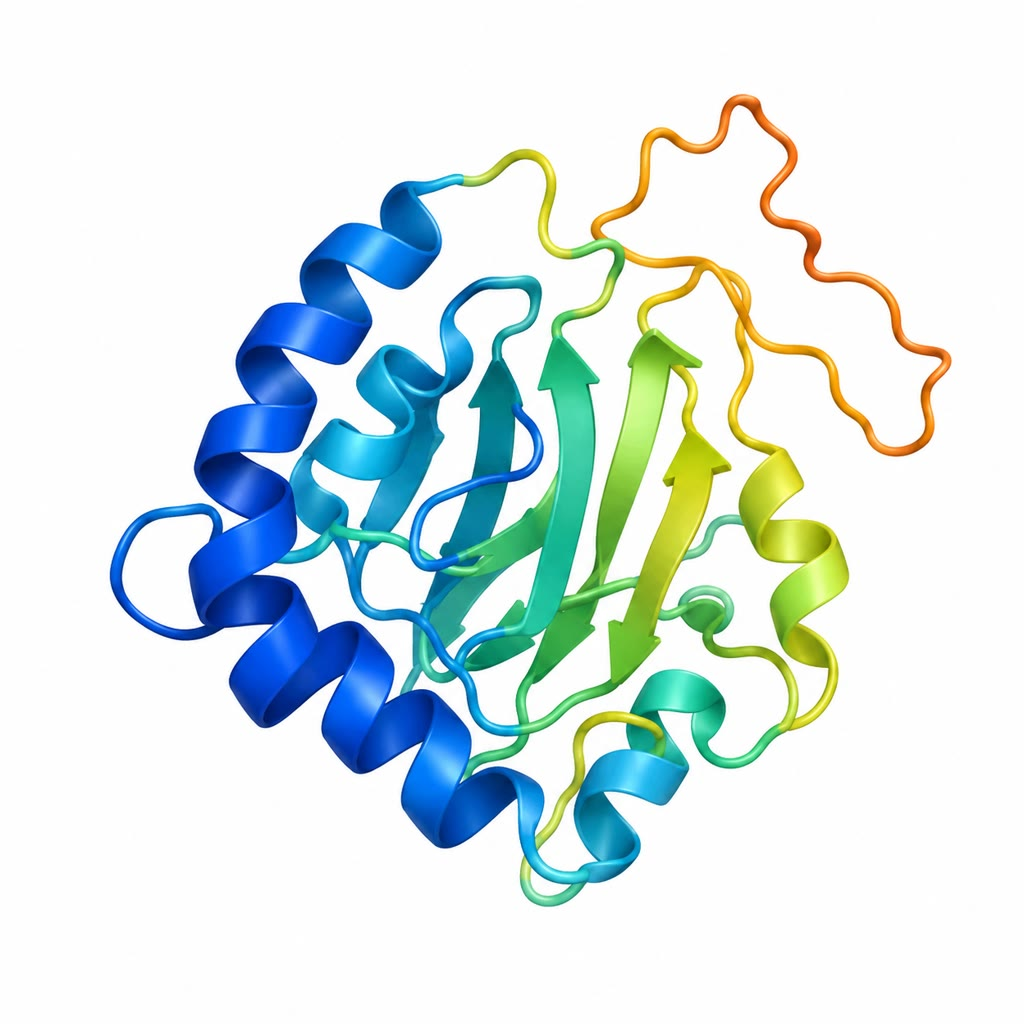
\includegraphics[width=0.36\linewidth]{images/book5/ai/b5-05-alphafold.jpg}\hspace{0.04\linewidth}
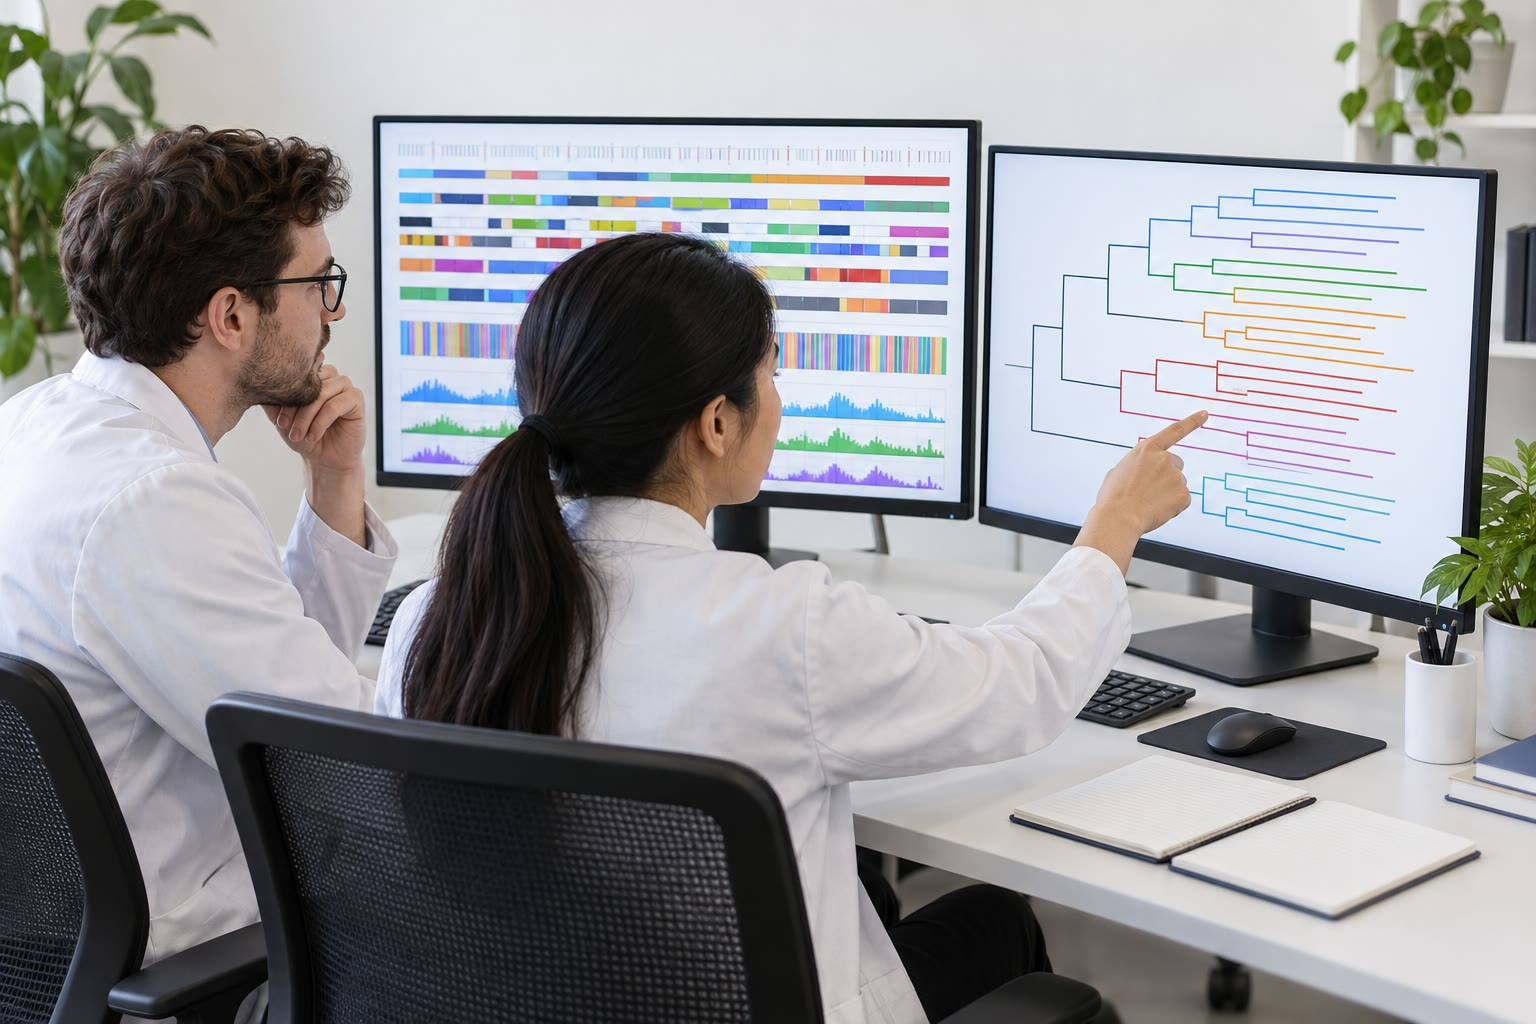
\includegraphics[width=0.54\linewidth]{images/book5/ai/b5-05-bioinformatics-lab.jpg}

{\small يسارًا: بنية بروتين متوقَّعة، ملوّنة بحسب ثقة النموذج
من العالية (بالأزرق) إلى المنخفضة (بالبرتقالي) في عروة غير منتظمة.
يمينًا: مكتب معلوماتية حيوية --- متصفحات جينوم وأشجار على
الشاشات، ولا أثر لمنضدة رطبة.}
\end{omfigure}

\begin{remark}[حدود الاستدلال]\label{rem:b3:bioinformatics:limits}
معظم التوصيفات الوظيفية في قواعد البيانات لم يُختبر قط؛ بل
نُقلت من متماثل كان قد وُصف هو بدوره
بالنقل. والأخطاء تنتشر وتتضاعف، والتوصيف الخاطئ على
بروتين كثير الوصلات قد يعدي أسرة كاملة. والعلاج هو ما
سبق: ميّز التعامد من التماثل، واقرأ \omterm{def:b3:bioinformatics:alignment}{المحاذاة}،
وابحث عن البقايا الحفّازة، واذكر أن ``بروتين
افتراضي'' وسم صادق ما يزال يستحقه ثلث المورّثات في معظم الجينومات.
\end{remark}

\section{تمارين}

\begin{exercise}[$\star$]\label{exo:b3:bioinformatics:1}
عرّف \omterm{def:b3:bioinformatics:alignment}{المحاذاة الشاملة} والموضعية وأعطِ لكل منهما حالة بيولوجية
واحدة تستدعيها.
\end{exercise}

\begin{exercise}[$\star$]\label{exo:b3:bioinformatics:2}
املأ جدول نيدلمان--فونش للمتتالية AGC في مواجهة AAC بمطابقة $+1$،
وعدم مطابقة $-1$، وفجوة $-1$، وأعطِ \omterm{def:b3:bioinformatics:alignment}{المحاذاة} المثلى ودرجتها.
\end{exercise}

\begin{exercise}[$\star$]\label{exo:b3:bioinformatics:3}
في BLOSUM62 تبلغ درجة تربتوفان--تربتوفان $+11$ ودرجة لوسين--لوسين
$+4$. فسّر من صيغة لوغاريتم الأرجحية لماذا يساوي تطابق البقية
الأندر أكثر.
\end{exercise}

\begin{exercise}[$\star$]\label{exo:b3:bioinformatics:4}
ما \omterm{thm:b3:bioinformatics:evalue}{القيمة المتوقعة E}؟ ويعطي بحث إصابة عند $E = 3$. فماذا يعني ذلك
العدد، وهل الإصابة متماثل؟
\end{exercise}

\begin{exercise}[$\star\star$]\label{exo:b3:bioinformatics:5}
يُبحث استعلام من \num{400} بقية في مواجهة $2\times 10^{11}$
بقية. احسب القيمة المتوقعة لإصابات درجات بتّاتها $45$ و$55$ و
$65$. وأي درجة بتّات تعطي $E = 10^{-3}$؟ وكيف يتغير الجواب
إذا كان طول الاستعلام \num{40} بقية؟
\end{exercise}

\begin{exercise}[$\star\star$]\label{exo:b3:bioinformatics:6}
احسب \omterm{def:b3:bioinformatics:motif}{المحتوى المعلوماتي} \omterm{def:b3:bioinformatics:motif}{لنميطة} مواضعها الأربعة تواترات قواعدها
(A وC وG وT) هي $(1,0,0,0)$ و$(0.5,0,0.5,0)$ و
$(0.25,0.25,0.25,0.25)$ و$(0.7,0.1,0.1,0.1)$. وكم مطابقة مصادفة
لها في جينوم قدره \qty{4.6}{Mb}؟
\end{exercise}

\begin{exercise}[$\star\star$]\label{exo:b3:bioinformatics:7}
فسّر لماذا تكون جزاءات الفجوة التآلفية أقرب إلى الواقع من الخطية،
ولماذا يعطي جزاء فتح عالٍ جدًا وجزاء منخفض جدًا محاذيات
رديئة كلاهما.
\end{exercise}

\begin{exercise}[$\star\star$]\label{exo:b3:bioinformatics:8}
يعطي بحث \omterm{def:b3:bioinformatics:blast}{BLAST} لبروتين بشري في قاعدة بيانات ذبابة أفضل
إصابة عند $E = 10^{-30}$ تغطي البقايا 50--180 من الاستعلام البالغ
\num{600} بقية. فهل بروتين الذبابة \omterm{def:b3:genomics:comparative}{متماثل متعامد} للبروتين البشري؟
وأي اختبار آخر تجريه؟
\end{exercise}

\begin{exercise}[$\star\star$]\label{exo:b3:bioinformatics:9}
لماذا تكشف طرائق الملامح متماثلات تفوت \omterm{def:b3:bioinformatics:alignment}{المحاذاة} الثنائية؟
أعطِ مثالًا على نمط عمود يلتقطه \omterm{def:b3:bioinformatics:msa}{الملمح} ولا تلتقطه
متتالية مفردة.
\end{exercise}

\begin{exercise}[$\star\star\star$]\label{exo:b3:bioinformatics:10}
بيّن أنه في نظام تدريج درجته المتوقعة موجبة، تكون درجة
\omterm{def:b3:bioinformatics:alignment}{محاذاة} سميث--ووترمان الموضعية لمتتاليتين عشوائيتين طويلتين
نامية خطيًا مع طولهما، وفسّر لماذا يجعل هذا نظرية
القيمة المتوقعة تخفق. وماذا يعني ذلك \omterm{def:b3:bioinformatics:alignment}{لمحاذاة} DNA بمطابقة
$+1$ وعدم مطابقة $-1$ عند محتوى \qty{60}{\%} من G وC؟
\end{exercise}

\begin{exercise}[$\star\star\star$]\label{exo:b3:bioinformatics:11}
يحتاج جدول نيدلمان--فونش إلى $mn$ خلية ذاكرة؛ ولصبغيين بطول
\qty{100}{Mb} ذلك $10^{16}$. صِف فكرتين يتجنب بهما
مُحاذو الجينومات ذلك (البذور والتسلسل؛ والتنطيق)، وما الذي تتخلى عنه
كل منهما.
\end{exercise}

\begin{exercise}[$\star\star\star$]\label{exo:b3:bioinformatics:12}
نموذج ماركوف مخفي للبحث عن المورّثات في البكتيريا له حالات لمواضع
الرامزة الثلاثة ولجزيء DNA غير المشفِّر. فسّر كيف يستطيع النموذج تمييز
التسلسل المشفِّر من غير المشفِّر بلا أي معلومة عن رامزات الوقف
(انظر انحياز الرامزات)، ولماذا يكون المسلك نفسه أصعب بكثير في
جينوم بشري.
\end{exercise}

\section{مسألة: متتالية من أعماق البحر}

\begin{problem}[{مسألة نهاية الأسبوع --- بروتين مجهول يُحاذى باليد،
ويُبحث في قواعد البيانات مع حساب دلالته، وتُوزن نميطته
التنظيمية بالبتّات، وتُقاس مورّثته في مواجهة إحصاء أطر القراءة
المفتوحة العشوائية، وتنتهي إلى القيمة المتوقعة لأفضل إصابة،
والبتّات التي يحتاجها موقع، والطول الذي يجب أن يبلغه إطار قراءة
حتى يُصدَّق}]
\label{pb:b3:bioinformatics:1}
معطيات: بروتين من \num{300} بقية من حلقية من أعماق البحر. وقاعدة
بيانات البروتينات: $1.2\times 10^{11}$ بقية. وجينوم الدودة:
\qty{1.6}{Gb}، و\qty{38}{\%} منه G وC. والتدريج في \omterm{def:b3:bioinformatics:alignment}{المحاذاة} اليدوية: مطابقة $+1$،
وعدم مطابقة $-1$، وفجوة $-1$. ودرجة بتّات أفضل إصابة \omterm{def:b3:bioinformatics:blast}{BLAST}: $92$؛ ودرجة
الإصابة العاشرة: $38$.

\medskip
\noindent\textbf{الجزء الأول --- باليد.}
\begin{enumerate}
  \item حاذِ الببتيدين KQT وKAQT بعلاقة تكرار
        نيدلمان--فونش: اكتب الجدول وأعطِ \omterm{def:b3:bioinformatics:alignment}{المحاذاة} المثلى
        ودرجتها.
  \item أعد ذلك بطريقة سميث--ووترمان (الموضعية) للمتتالية GATCAT في مواجهة ACAT:
        أوجد أفضل \omterm{def:b3:bioinformatics:alignment}{محاذاة موضعية} ودرجتها.
  \item كم تحديث خلية تقتضي \omterm{def:b3:bioinformatics:alignment}{محاذاة شاملة} للبروتين البالغ
        \num{300} بقية في مواجهة بروتين من \num{450} بقية؟
        وفي مواجهة قاعدة البيانات كلها؟
  \item إذا نفّذ حاسوب $10^{9}$ تحديث في الثانية، فكم
        تستغرق \omterm{def:b3:bioinformatics:alignment}{محاذاة} قاعدة البيانات كاملةً في السؤال 3؟ ولماذا
        تُستعمل \omterm{def:b3:bioinformatics:blast}{BLAST} بدلًا منها؟
  \item درجة التطابق في BLOSUM62 هي $+4$ للألانين ($p_{A} =
        0.074$) و$+11$ للتربتوفان ($p_{W} = 0.013$). وعند
        $\lambda = 0.347$ (بوحدات نصف البتّ)، احسب التواتر
        الهدف $q_{AA}$ وَ$q_{WW}$، والنسبة $q/p^{2}$ لكل
        منهما. وفسّر.
  \item يشترك بروتينان في \qty{24}{\%} تطابقًا على $250$ بقية.
        قل لماذا لا يستطيع التطابق وحده أن يحسم التماثل هنا وما
        الذي يحسمه.
\end{enumerate}

\medskip
\noindent\textbf{الجزء الثاني --- البحث.}
\begin{enumerate}[resume]
  \item احسب $mn$ للاستعلام في مواجهة قاعدة البيانات، و
        $\log_{2}(mn)$.
  \item احسب القيمة المتوقعة لأفضل إصابة ($S' = 92$) وللإصابة
        العاشرة ($S' = 38$).
  \item أي درجة بتّات توافق $E = 10^{-3}$ في هذا البحث؟
        وأيها توافق $E = 1$؟
  \item تُوجد أفضل إصابة نفسها بعد أن كبرت قاعدة البيانات إلى
        $1.2\times 10^{12}$ بقية. فما قيمتها المتوقعة؟
  \item تحاذي الإصابة العاشرة البقايا 200--260 من الاستعلام بتطابق
        \qty{40}{\%} على $60$ بقية. باستعمال القيمة المتوقعة،
        قل هل هي دليل تماثل، وما الذي يضيفه بحث
        بالملامح.
  \item أفضل إصابة كيناز بشري، محاذًى على البقايا 10--290.
        وأفضل إصابة له في مجموع بروتينات الدودة هي الاستعلام. فما الذي
        يثبته هذا المحك المتبادل، وما الذي لا يثبته؟
\end{enumerate}

\medskip
\noindent\textbf{الجزء الثالث --- \omterm{def:b3:bioinformatics:motif}{نميطة}.}
\begin{enumerate}[resume]
  \item أعلى المورّثة يقع موقع مرشح لعامل استنساخ
        من ثمانية مواضع محتوياتها المعلوماتية
        $2, 2, 1.6, 2, 0.8, 1.2, 0.4, 0.3$ بتّ. فما المجموع $R$؟
  \item كم مطابقة مصادفة \omterm{def:b3:bioinformatics:motif}{للنميطة} في الجينوم البالغ
        \qty{1.6}{Gb} (على الطاقين، أي $3.2\times 10^{9}$
        موضع)؟
  \item ينظم العامل نحو $200$ مورّثة. فكم بتًّا تحتاج
        نميطةٌ لتحدد $200$ موقع وحدها في هذا الجينوم؟
  \item كم من النقص تستطيع \omterm{def:b3:bioinformatics:motif}{نميطة} ثانية مجاورة من
        $8$ بتّات أن تسدّ، إذا وجب أن تردا معًا ضمن مباعدة
        ثابتة؟
  \item موضع تواتراته $(0.5, 0.5, 0, 0)$ في (A وC وG و
        T): احسب إنتروبيته ومحتواه المعلوماتي.
  \item فسّر، بحجة المعلومات، لماذا تكون مواقع عوامل
        الاستنساخ البكتيرية أطول وأشد حفظًا عادةً من مواقع
        عوامل حقيقيات النوى.
\end{enumerate}

\medskip
\noindent\textbf{الجزء الرابع --- المورّثة نفسها.}
\begin{enumerate}[resume]
  \item في DNA عشوائي متساوي تركيب القواعد، ما
        احتمال أن تكون الرامزة رامزةَ وقف؟ وما العدد
        المتوقع من الرامزات قبل ظهور وقف (توزيع
        هندسي)؟
  \item جينوم الدودة \qty{38}{\%} منه G وC. أعد حساب احتمال
        أن تكون رامزة عشوائية رامزةَ وقف (TAA أو TAG أو TGA) بتواترات
        القواعد الفعلية، والطول المتوقع لإطار القراءة. وفي أي
        اتجاه يدفع محتوى G وC المنخفض البحثَ عن المورّثات؟
  \item ما احتمال أن يكون إطار قراءة مفتوح عشوائي بطول
        $100$ رامزة على الأقل؟ وبطول $300$ على الأقل؟
  \item في الجينوم البالغ \qty{1.6}{Gb}، تعطي ستة أطر على طاقين
        نحو $3.2\times 10^{9}$ بداية رامزة. فكم إطار قراءة مفتوحًا
        عشوائيًا بطول $100$ رامزة على الأقل يُتوقع؟ وبطول
        $300$ على الأقل؟
  \item فسّر لماذا يكون ``إطار قراءة مفتوح أطول من $100$ رامزة''
        كاشفًا صالحًا للمورّثات في بكتيريا لا في هذا الجينوم،
        وما الذي يستعمله كاشف المورّثات في حقيقيات النوى بدلًا منه.
  \item لمورّثة الدودة ستة إكسونات متوسطها \qty{150}{bp}. فسّر
        كيف تحلّ قراءات تسلسل RNA بنية الإكسونات التي يتركها
        التسلسل الجينومي وحده ملتبسة.
  \item لخّص: القيمة المتوقعة لأفضل إصابة (السؤال~8)، والبتّات
        اللازمة لتحديد $200$ موقع (السؤال~15)، والعدد المتوقع
        من أطر القراءة العشوائية بطول $300$ رامزة في الجينوم
        (السؤال~22).
\end{enumerate}
\end{problem}
